В данной главе рассмотрена искусственная нейронная сеть, которая использует архитектуру трансформера для генерации продолжения композиций.
Перед тем как приступить к изложению архитектуры Theme Transformer \cite{theme}, стоит объяснить архитектуру классических трансформеров, и только потом перейти к его модификации.

\section{ОПИСАНИЕ АРХИТЕКТУРЫ ТРАНСФОРМЕРОВ}
\subsection{ОСНОВНАЯ ИДЕЯ МОДЕЛИ}
    Большинство seq2seq моделей основаны на больших рекуррентных или сверточных нейронных сетях, которые включают в себя кодировщик и декодер. Лучшего результата таких моделей можно достичь, если кодировщик и декодер будут соединены между собой механизмом внимания. В статье представлена модель трансформера, основанного на архитектуре модели seq2seq, имеющий механизм внимания, что имеет преимущества \cite{attention}. Во-первых, нет необходимости иметь свёрточные и рекуррентные слои. Во-вторых, обучение модели может проходить параллельно. В-третьих, модели требуется меньше времени на тренировку.
    
    Данная архитектура (рисунок \ref{fig:transformer}) является модификацией архитектуры seq2seq модели. Модификация заключается в наличии в каждом кодировщике механизма самовнимания (self-attention) и классического механизма внимания (attention) между кодировщиком и декодером.
    
    \begin{figure}
        \centering
        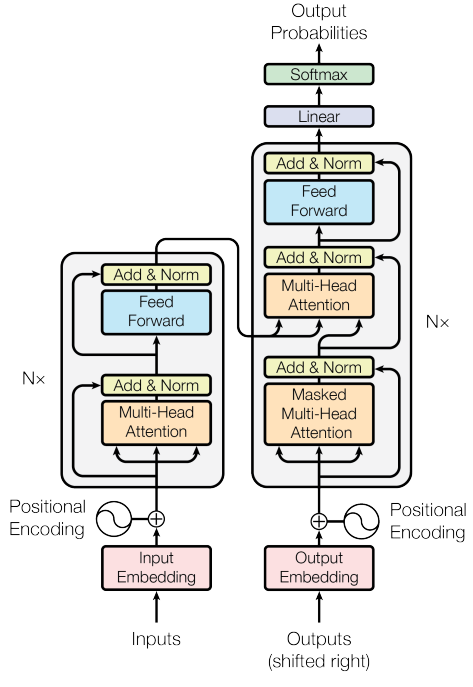
\includegraphics[scale=1.2]{tex/png/transformer.png}
        \caption{Архитектура трансформера \cite{attention}}
        \label{fig:transformer}
    \end{figure}
    
    Недостатком seq2seq модели является скрытый вектор состояния фиксированного размера, что не позволяет сжать много информации из ввода, особенно если он длинный.

    Механизм внимания позволяет отказаться от основной идеи рекуррентных и сверточных нейронных сетей, тем самым ускорив обучение нейронной сети, т. к. появляется возможность тренировать их независимо.

\subsection{АРХИТЕКТУРА}
    Кодировщики и декодеры представляют собой некоторый стек идентичных слоёв. 
    
    Каждый слой в кодировщике состоит из двух подслоёв. Первым слоем является multi-head self-attention механизм, а второй -- полносвязный. После них расположен слой нормализации, который принимает вход с предыдущего слоя (остаточная связь), то есть $ LayerNorm(x + Sublayer(x)) $, где $ Sublayer(x) $ -- это функция, которая реализуется слоем (в нашем случае это или multi-head self-attention, или полносвязный слои). Чтобы было легче пользоваться остаточной связью, каждый слой формирует вектор одинаковой размерности. 
    
    Если у кодировщика слой состоит из 2 подслоёв, то к декодеру добавляется третий multi-head attention, который принимает выход из кодировщика. Также этот слой принимает на вход результат слоя самовнимания, который маскирует некоторые позиции и, как следствие, игнорируются моделью. Эта маскировка и смещение выходного вектора на одну позицию гарантирует, что прогноз на $i$-й позиции зависит только от позиций меньших $i$.

\subsection{МЕХАНИЗМ ВНИМАНИЯ}
    Механизм внимания оперирует 3-я элементами: $Q$ -- запрос размерности $ d_k $, $K$ -- ключ размерности $ d_k $ и $V$ -- значение размерности $ d_v $.
    
    Данные элементы получаются в результате перемножения исходного вектора на матрицы $W^Q, W^K, W^V$ соответственно. Они формируются во время обучения нейронной сети и являются некоторым скрытым состоянием.
    
    Данный механизм в качестве элементов $Q, K, V$ может иметь вектора или матрицы.
    
    Вектор или матрица (в зависимости от вида механизма) внимания вычисляется следующим образом:
    $$ Attention(Q, K, V) = softmax(\frac{QK^T}{\sqrt{d_k}})V, $$
    где softmax -- функция вида $f(x) = \frac{\exp{x_k}}{\sum \exp{x_i}}$, $\frac{1}{\sqrt{d_k}}$ -- нормирующий коэффициент, который позволяет увеличить градиент (отчасти решая проблему исчезающих градиентов).
    
\subsection{MULTI-HEAD ATTENTION}
    Входной вектор разбивается на h частей. Таким образом, у каждого механизма внимания размерность следующая: $d_k = d_v = d_{model} / h$.
    
    В декодере один из таких механизмов должен принимать выход от кодировщика, ожидая от него $K$ и $V$. 
    
    Благодаря разбиению одного большого механизма внимания на несколько маленьких (в оригинальной статье разбивается на 8 частей) позволяет модели фокусироваться на разных частях входа \cite{attention}. Таким образом, модель способна выявлять связи между различными позициями.
    Также благодаря этому увеличивается количество подпространств. Это позволяет каждому маленькому механизму концентрироваться только на связи отдельных позиций.
    
    После того, как вектор прошёл через данный механизм, нам необходимо вернуться к исходному пространству векторов, так как полносвязный слой ожидает на вход вектор размерности $d_{model}$. Чтобы этого добиться, нам необходимо конкатенировать вектора с каждой головы (маленькая часть) и умножить на общую матрицу $W^O$ (формируется во время обучения).
    
    Формализуя описанные шаги, получаем:
    $$ MultiHead(Q, K, V) = Concat(head_1, ..., head_h)W^O, $$
    где $head_i = Attention(QW_{i}^Q, KW_{i}^K, VW_{i}^V)$, $Concat$ -- функция конкатенации векторов в один, $W_i^Q \in R^{d_{model} \times d_k}$, $W_i^K \in R^{d_{model} \times d_k}$, $W_i^V \in R^{d_{model} \times d_v}$, $W^O \in R^{hd_v \times d_{model}}$.
    
\subsection{СЕТИ ПРЯМОГО РАСПРОСТРАНЕНИЯ, ЗАВИСЯЩИЕ ОТ ПОЗИЦИИ}
    Каждый блок декодера и кодировщика содержит в себе полносвязную сеть прямого распространения, которая идентично применяется ко всем позициям отдельно. В нём содержится две линейные трансформации с функцией активации ReLU:
    $$ FFN(x) = max(0, xW_1 + b_1)W_2 + b2. $$
    
    Линейные преобразования одинаковы для разных позиций, но они имеют разные параметры от слоя к слою, что эквивалентно использованию двух сверточных слоёв с размером ядра 1. 
    

\section{ОПИСАНИЕ РАБОТЫ THEME TRANSFORMER}
    В последние годы стала популярна архитектура трансформеров, т.к. в ней используется механизм внимания (в частности self-attention), который обеспечивает модели гораздо большую память по сравнению с рекуррентной нейронной сетью.
    
    Такие модели всё чаще используют для генерации музыки. Популярным подходом, обуславливающим процесс генерации, является принятие входных данных как последовательности инициализации для дальнейшей работы декодера. 
    Данный метод не гарантирует развития и повторения элементов исходных данных в генерированном продолжении. 
    Однако данная модель, описанная далее, использует альтернативный подход ко входным данным. При добавлении входной последовательности система трактует её как тематический материал, который должен многократно проявляться в результате генерации.
    
    Приведённый выше подход реализуется с помощью метода, основанный на глубоком обучении. Он использует изучение контрастного представления и кластеризацию для автоматического извлечения тематических материалов из музыкальных произведений в обучающих данных. Также он необходим для выявления в композиции основной темы. Также модифицирована архитектура декодера: self-attention идёт параллельно cross-attention, после чего применяется операция XOR, полученные вектора суммируются и нормализуются. Данная модификация используется для более эффективного учёта заданного тематического материала в процессе генерации.

    По итогу данная модель может использоваться для генерации произведений с нуля или с подсказкой, предоставленной пользователем, для создания продолжения. 
    
    Генерация произведений с нуля возможна благодаря тому, что обучается модель трансформера, которая состоит из двух частей. Кодировщик обеспечивает некоторое внутреннее представление композиции, а декодер может взять выход с кодировщика или случайное начальное значение и генерировать продолжение.
    
    Такая архитектура позволяет изучать языковую модель музыки без правил, созданных вручную, и генерировать уникальные и разнообразные произведения, которые внутренне согласованы. Однако эта стратегия не гарантирует, что модель будет повторять или развивать данное условие или ранее созданный материал. Более того, поскольку музыкальное произведение постоянно расширяется, влияние начального фрагмента со временем уменьшается, т.е. модель теряет направление.
    
    \subsection{ПОДХОД К ОБУЧЕНИЮ}
    Рассмотрим подход к данным. Существуют уже готовые наборы данных и необходимо обучить модель, которая используя основную тему генерирует продолжение. И так как выделять самостоятельно в огромном наборе данных основную тему было бы крайне затратно -- реализован алгоритм, который делает это сам. 
    
    Суть алгоритма заключается в том, чтобы разбить исходную композицию на сегменты и получить их представление через кодировщик. Т. к. потом идёт работа с векторами -- в таком случае можем использовать алгоритм кластеризации (в оригинальной статье используется DBSCAN) для обнаружения наибольшего кластера. Первое вхождение в данный кластер и будет являться основной темой, а размер кластера будет указывать на частоту его появления в генерируемой композиции.
    
    После такой разметки данных модель обучается с использованием основной темы генерировать исходную композицию.
    
    \subsection{АРХИТЕКТУРА THEME TRANSFORMER}
    Архитектура Theme Transformer (рисунок \ref{fig:theme_transformer}) является модификацией исходного трансформера.
    В декодере изменён модуль внимания, в котором теперь cross attention не использует выход из самовнимания, а идёт параллельно. 
    При этом в архитектуре используется операция XOR для двух векторов. 
    После этого они подаются на вход нормировки и в сеть прямого распространения.
    
    Данное изменение улучшает работу при генерировании с условием \cite{theme}. 
    \begin{figure}[h]
        \centering
        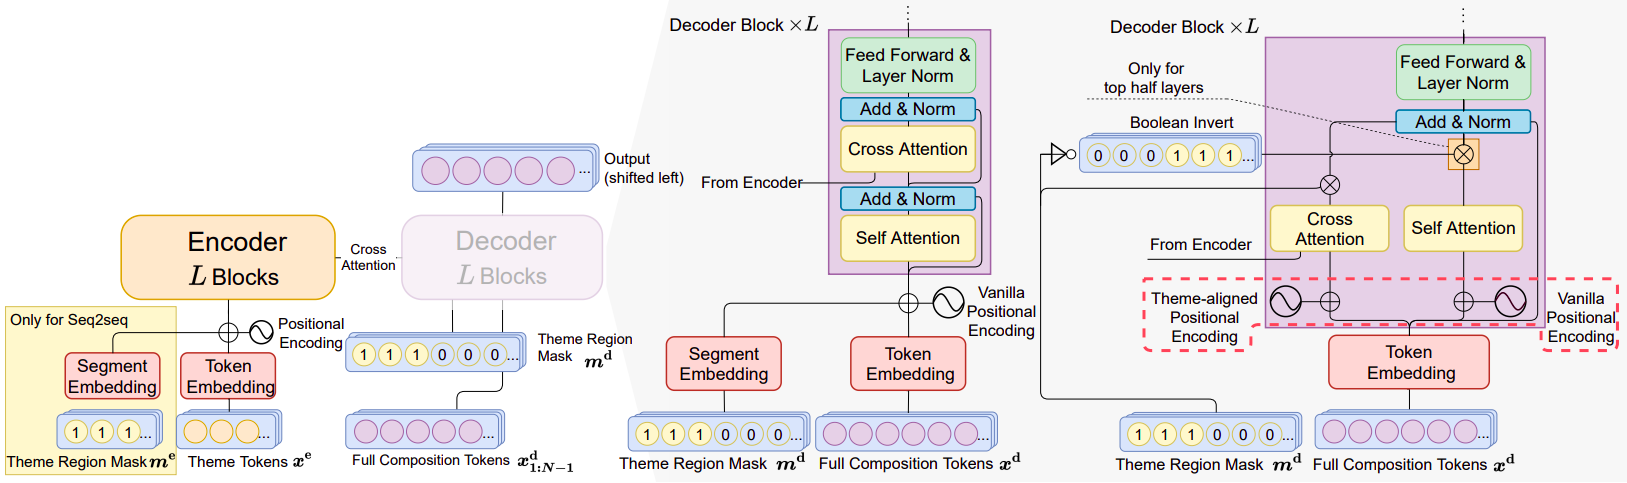
\includegraphics[scale=0.3]{tex/png/theme_transformer.png}
        \caption{Архитектура Theme Transformer с наглядной демонстрацией отличий от классической seq2seq модели \cite{theme}}
        \label{fig:theme_transformer}
    \end{figure}
    
    \subsection{ПРОЦЕСС ОБУЧЕНИЯ}
    
    Обучение происходит на основе набора данных POP909, состоящего из популярных композиций, которые исполняют только на пианино. Они созданы профессиональными музыкантами. Каждый MIDI-файл состоит из трёх дорожек: MELODY (основная мелодия, которую исполняет вокал), BRIDGE (второстепенная мелодия или основной инструмент) и PIANO (основной аккомпанемент). Для изучаемой модели дорожка BRIDGE была опущена, т. к. включает в себя функции и MELODY, и PIANO. Игнорирование названной дорожки не сильно ухудшает качество исходных треков \cite{theme}.
    
    Были выбраны композиции с тактовым размером 4/4. Также ноты были выравнены таким образом, чтобы время их начала и длительность были кратны 1/4 доли. Таким образом были проигнорированы сложные приёмы построения ритмических рисунков с целью упрощения работы модели. Также были убраны композиции с модуляцией.
    
    В итоге набор состоит из 713 композиций. 4\% оставлены для тестирования (29 файлов), а остальные -- для обучения модели. 

    Рассматриваются три вида токенов для представления каждой песни из POP909: для описания ноты, для описания звучания по времени, для описания начала и конца `основной темы`.
    
    Каждая нота в песне состоит из трёх лексем: высота (NOTE-PITCH; от D0 до G9), длительность (NOTE-DURATION; от 1/4 до 16 долей, кратная 1/4) и сила исполнения (NOTE-VELOCITY; от 1 до 126). Также необходимо принимать несколько дорожек; соответственно, будет использован отдельный токен, обозначающий мелодию или аккомпанемент. Например, чтобы описать высоту ноты дорожки MELODY в C5, используется токен NOTE-PITCH:MELODY:C5. 
    
    Для представления звучания по времени используются токены, связанные с метрикой. BAR отмечает начало нового такта, равномерно разделенного на 16 частей. SUBBEAT указывает время начала ноты среди этих 16 возможных позиций в такте. TEMPO описывает скорость песни на уровне битов и принимает значения от 17 до 194 ударов в минуту с интервалом 3. 
    
    Всего словарь для фортепиано содержит 730 уникальных токенов. Среди них нет токена конца композиции, т.к. используется последовательность из 512-ти токенов на вход вместо передачи всей композиции, что позволяет генерировать продолжение бесконечно.
    
    В тренировочном наборе данных композиции имеют в среднем 95 тактов, что составляет 5 249 токенов на песню с использованием представления фортепиано. Соответственно, последовательность из 512 токенов, используемая при обучении модели, содержит в среднем около девяти тактов. Фрагмент с основной темой из двух тактов содержит в среднем 122 токена.
    
